\begin{document}
The design of the CMOS ring oscillator consists of three CMOS inverters connected in series with the
output of the last inverter connected to the input of the first inverter. The ring oscillator will also have a
capacitor at each output connected to ground. The schematic for the CMOS ring oscillator can be seen in
Figure 20.


\begin{figure}[H]
	\centering
	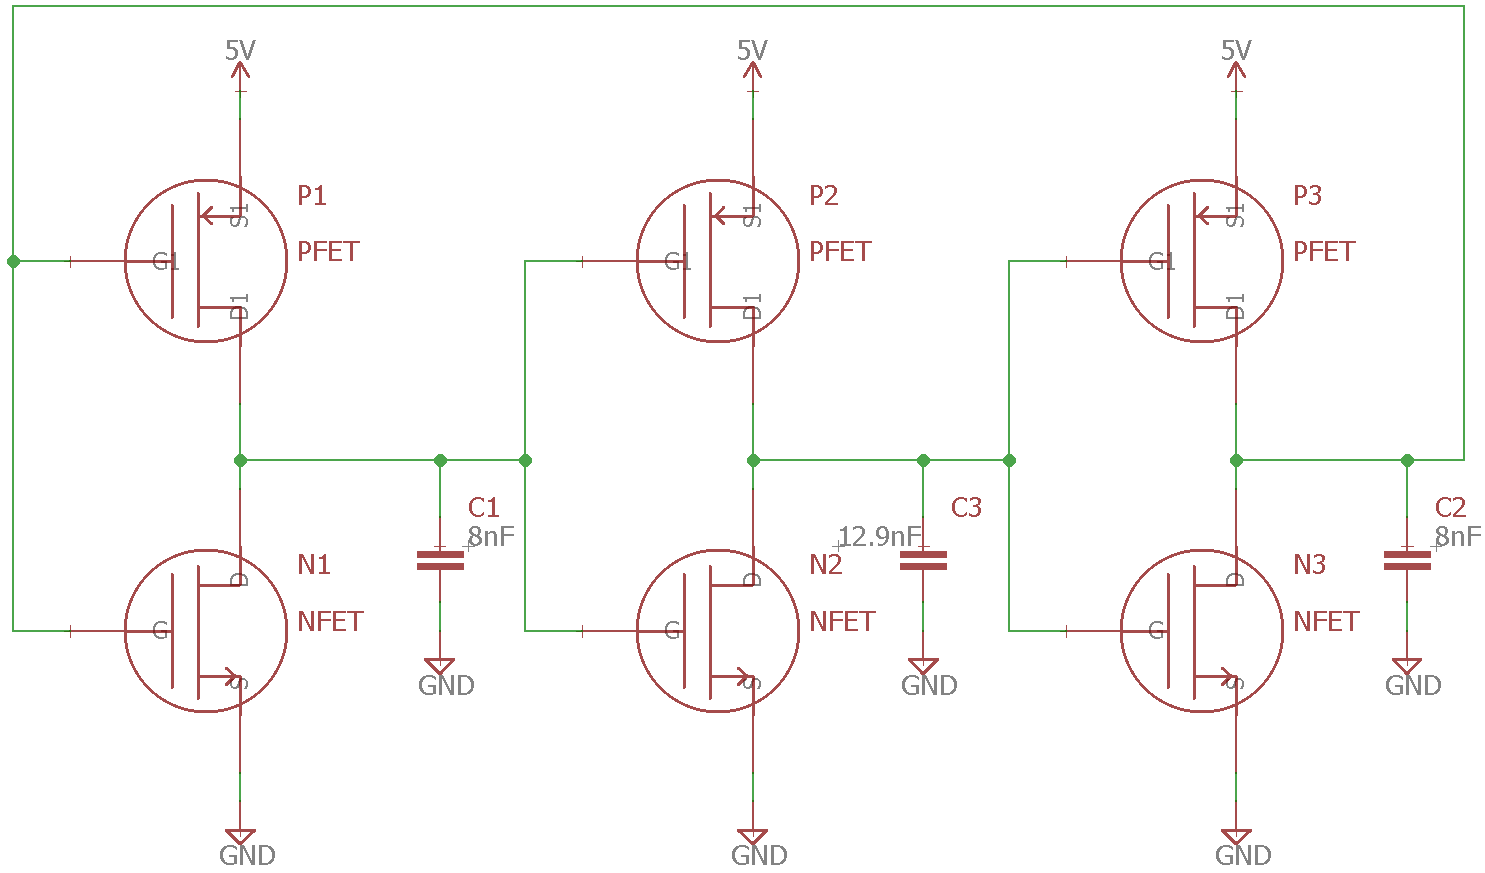
\includegraphics[width=0.5\linewidth]{CircuitDevelopment/RingOscillatorCMOSexp.png}
	\caption{}
	\label{fig:ringoscillatorcmosexp}
\end{figure}


The operation of the ring oscillator uses a series of inverters. The output of one inverter inverts the input signal. Therefore, if there are a series of inverters, then each odd inverter will have the same inverted output as the first. In this instance, there are three stages of inverters used, with the output of the third inverter being fed back into the input of the first inverter. This feedback from the output to the input causes an oscillation.

The ring oscillator circuit requires only a DC power source with a threshold voltage above what is required of the MOSFETS, and the oscillations will occur. To increase the frequency, the DC supply can be increased, causing an increase in current as well as frequency. The inverse of the oscillation frequency, the oscillation period, is based on the delay in each stage of the
ring oscillator. The period is equivalent to double the sum of all propagation delays. These delays are
caused by gates being unable to switch instantly in the real world. In this case, the gate capacitance must be charged before a connection is made between the source and the drain. Otherwise, current will be un-
able to flow between the source and the drain. The time it takes for the gate capacitance to reach the necessary charge adds a delay to the oscillator. Increasing the number of stages increases the delay time and

\end{document}